

\tikzset{every picture/.style={line width=0.75pt}} %set default line width to 0.75pt        

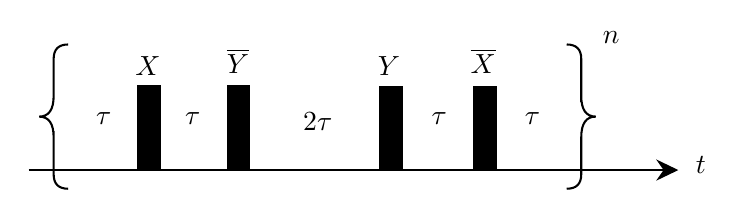
\begin{tikzpicture}[x=0.75pt,y=0.75pt,yscale=-1,xscale=1]
%uncomment if require: \path (0,300); %set diagram left start at 0, and has height of 300

%Straight Lines [id:da6050772876669203] 
\draw    (113.5,159.5) -- (423.5,159.5) ;
\draw [shift={(426.5,159.5)}, rotate = 180] [fill={rgb, 255:red, 0; green, 0; blue, 0 }  ][line width=0.08]  [draw opacity=0] (10.72,-5.15) -- (0,0) -- (10.72,5.15) -- (7.12,0) -- cycle    ;
%Shape: Rectangle [id:dp03677959381184914] 
\draw  [fill={rgb, 255:red, 0; green, 0; blue, 0 }  ,fill opacity=1 ] (166,119) -- (176.5,119) -- (176.5,159) -- (166,159) -- cycle ;
%Shape: Rectangle [id:dp9515559699003447] 
\draw  [fill={rgb, 255:red, 0; green, 0; blue, 0 }  ,fill opacity=1 ] (209.33,119) -- (219.83,119) -- (219.83,159) -- (209.33,159) -- cycle ;
%Shape: Rectangle [id:dp3750218499878627] 
\draw  [fill={rgb, 255:red, 0; green, 0; blue, 0 }  ,fill opacity=1 ] (282.66,119.5) -- (293.16,119.5) -- (293.16,159.5) -- (282.66,159.5) -- cycle ;
%Shape: Rectangle [id:dp4039169654303607] 
\draw  [fill={rgb, 255:red, 0; green, 0; blue, 0 }  ,fill opacity=1 ] (328,119.5) -- (338.5,119.5) -- (338.5,159.5) -- (328,159.5) -- cycle ;
%Shape: Brace [id:dp43500153185683443] 
\draw   (132.51,99) .. controls (127.84,99) and (125.51,101.33) .. (125.51,106) -- (125.51,123.75) .. controls (125.51,130.42) and (123.18,133.75) .. (118.51,133.75) .. controls (123.18,133.75) and (125.51,137.08) .. (125.51,143.75)(125.51,140.75) -- (125.51,161.5) .. controls (125.51,166.17) and (127.84,168.5) .. (132.51,168.5) ;
%Shape: Brace [id:dp32462909095886316] 
\draw   (372.71,168.5) .. controls (377.38,168.5) and (379.71,166.17) .. (379.71,161.5) -- (379.71,143.75) .. controls (379.71,137.08) and (382.04,133.75) .. (386.71,133.75) .. controls (382.04,133.75) and (379.71,130.42) .. (379.71,123.75)(379.71,126.75) -- (379.71,106) .. controls (379.71,101.33) and (377.38,99) .. (372.71,99) ;

% Text Node
\draw (433.5,151.4) node [anchor=north west][inner sep=0.75pt]    {$t$};
% Text Node
\draw (170.94,109.19) node    {$X$};
% Text Node
\draw (214.27,107.19) node    {$\overline{Y}$};
% Text Node
\draw (287.1,109.19) node    {$Y$};
% Text Node
\draw (332.44,107.19) node    {$\overline{X}$};
% Text Node
\draw (144.5,130.4) node [anchor=north west][inner sep=0.75pt]    {$\tau $};
% Text Node
\draw (187.38,130.4) node [anchor=north west][inner sep=0.75pt]    {$\tau $};
% Text Node
\draw (244.26,130.4) node [anchor=north west][inner sep=0.75pt]    {$2\tau $};
% Text Node
\draw (306.14,130.4) node [anchor=north west][inner sep=0.75pt]    {$\tau $};
% Text Node
\draw (351,130.4) node [anchor=north west][inner sep=0.75pt]    {$\tau $};
% Text Node
\draw (388.69,91.4) node [anchor=north west][inner sep=0.75pt]    {$n$};


\end{tikzpicture}
